\chapter[Tecnlogias de Processo]{Tecnlogias de Processo}
\label{chap:tecnologias}
	
	\section[Definição]{Definição}
	\label{sec:tecnologias_definicao}

		Frequentemente, as discussões acerca do Gerenciamento de Processos são marcadas pelo ponto chave "Tecnologia", de modo que temos uma prática focada nos processos e suportada por plataformas tecnológicas, ocorrendo assim uma integração entre os fatores negócios e tecnologias. 

		\begin{figure}[h]
			\centering
			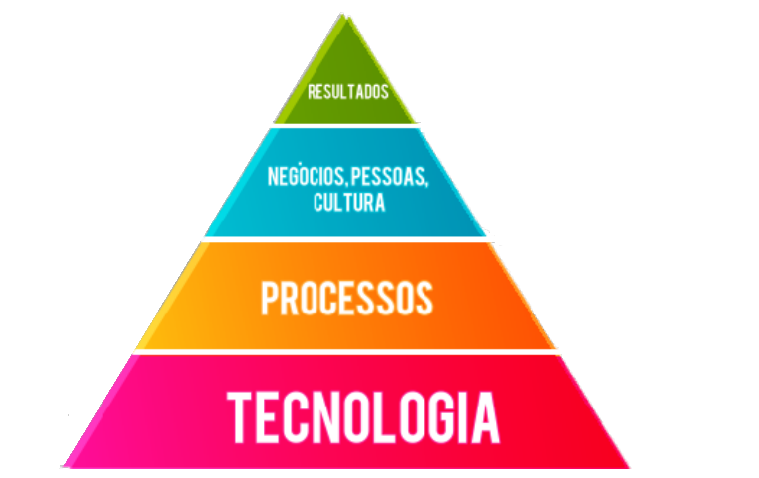
\includegraphics[scale=0.6]{tec1}
			\caption[O que suporta os resultados]{O que suporta os resultados.}
			\label{fig:suporta_resultados}
		\end{figure}


		Assim, a tecnologia auxiliará na hora de adequar os processos aos objetivos gerais da organização, gerando uma maior eficácia, eficiência e competitividade. Considerando ainda o nível de complexidade das tarefas e dinamicidade das mudanças, há uma necessidade de utilizar as tecnologias para a performance da organização, no quesito automatização de atividades e na integração de sistemas, indivíduos e ações.

		\subsection[Tecnologia de processamento de Materiais]{Tecnologia de processamento de Materiais}
		\label{sec:tecnologias_definicao_materiais}

			TO DO

		\subsection[Tecnologia de processamento de Informações]{Tecnologia de processamento de Informações}
		\label{sec:tecnologias_definicao_informacoes}
		
			TO DO

		\subsection[Tecnologia de processamento de Consumidores]{Tecnologia de processamento de Consumidores}
		\label{sec:tecnologias_definicao_consumidores}

			TO DO

	\section[Gerenciamento de operações e tecnologia de processo]{Gerenciamento de operações e tecnologia de processo}
	\label{sec:tecnologias_Gerenciamento}
		
		Os responsáveis pelo gerenciamento de tecnologias de processo são os gerentes da produção e os mesmos precisam ter a capacidade de se relacionarem com a tecnologia em si sabendo as melhorias que podem ser causadas nas operações, integrar a tecnologia com a produção, monitorando o desempenho e atualizar ou substituir a tecnologia em caso de necessidade.
		
		Não é necessário que os gerentes da produção sejam expert em alguma área específica, somente que saibam aplicar os conceitos de gestão e garantia de qualidade de modo que a performance de qualquer corporação seja impulsionado, utilizando os princípios apresentados pela norma NBR ISO 9000:

		\begin{itemize}
			\item{Envolvimento dos indivíduos: pelo fato de uma corporação ser composta por várias pessoas com um ou vários objetivos pré-determinados, o envolvimento dessas pessoas no processo de assimilação das políticas de qualidade é necessário para interagir e inserir as mesmas na organização, aproveitando as habilidades individuais;}
			\item{Liderança: os gerentes da produção ou líderes devem ser capazes de envolver as pessoas e entender a importância da gestão de qualidade e seus processos;}
			\item{Foco no cliente: "É recomendável que os requisitos organizacionais sejam motivados a atender e exceder as expectativas dos clientes.";}
			\item{Relacionamento com fornecedores: esse relacionamento deve possuir o benefício mútuo e a ampliação da capacidade de geração de valor agregado pela parceria como foco;}
			\item{Melhoria Contínua: a busca por uma constante melhoria no desempenho global deve ser considerado como um objetivo permanente. Um bom exemplo é o ciclo PDCA, que prevê o constante planejamento e re-planejamento de ações.}
		\end{itemize}

		\begin{figure}[h]
			\centering
			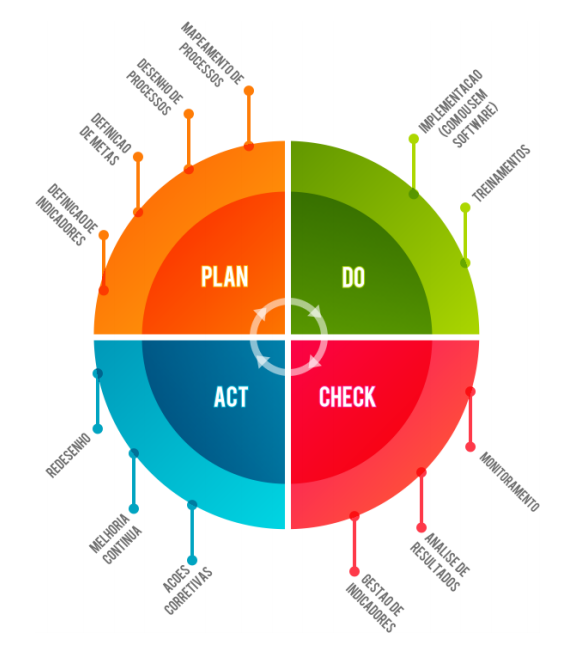
\includegraphics[scale=0.6]{tec2}
			\caption[Ciclo PDCA (Plan - Planejar, Do - Fazer, Check - Checar e Act - Agir) ]{Ciclo PDCA (\emph{Plan} - Planejar, \emph{Do} - Fazer, \emph{Check} - Checar e \emph{Act} - Agir) }
			\label{fig:cicloPDCA}
		\end{figure}

		Além desses princípios, os gerentes da produção devem ser capazes de lidar com os experts de tecnologia e realizar algumas perguntas para fazer um estudo acerca da tecnologia que será utilizada: 

		\begin{itemize}
			\item{O que a tecnologia é capaz de fazer? Qual a diferença entre ela e as outras tecnologias similares?}
			\item{Quais características particulares da tecnologia são usadas para realizar suas respectivas funções?}
			\item{Quais são os benefícios que a tecnologia pode oferecer?}
			\item{Quais são as limitações impostas pela tecnologia?}
		\end{itemize}

	\section[Tecnologia aplicada nas redes de fast-food do Bob's]{Tecnologia aplicada nas redes de fast-food do Bob's}
	\label{sec:tecnologias_aplicadas}

		TO DO
	